\documentclass{article}

\usepackage{algorithm}
\usepackage{algpseudocode}
\usepackage{appendix}
\usepackage{amsmath}
\usepackage{amssymb}
\usepackage[UTF8]{ctex}
\usepackage{fancyhdr}
\usepackage{float}
\usepackage{graphicx}
\usepackage{listings}
\usepackage{multirow}
\usepackage{tabularx}
\usepackage{newclude}
\usepackage{subfig}
\usepackage{xcolor}

\lstset{
    basicstyle          =   \sffamily,          % 基本代码风格
    keywordstyle        =   \bfseries,          % 关键字风格
    commentstyle        =   \rmfamily\itshape,  % 注释的风格,斜体
    stringstyle         =   \ttfamily,  % 字符串风格
    flexiblecolumns,                % 别问为什么,加上这个
    numbers             =   left,   % 行号的位置在左边
    showspaces          =   false,  % 是否显示空格,显示了有点乱,所以不现实了
    numberstyle         =   \zihao{-5}\ttfamily,    % 行号的样式,小五号,tt等宽字体
    showstringspaces    =   false,
    captionpos          =   t,      % 这段代码的名字所呈现的位置,t指的是top上面
    frame               =   lrtb,   % 显示边框
}

\lstdefinestyle{Python}{
    language        =   Python, % 语言选Python
    basicstyle      =   \zihao{-5}\ttfamily,
    numberstyle     =   \zihao{-5}\ttfamily,
    keywordstyle    =   \color{blue},
    keywordstyle    =   [2] \color{teal},
    stringstyle     =   \color{magenta},
    commentstyle    =   \color{red}\ttfamily,
    breaklines      =   true,   % 自动换行,建议不要写太长的行
    columns         =   fixed,  % 如果不加这一句,字间距就不固定,很丑,必须加
    basewidth       =   0.5em,
}

\title{计算机视觉——第一次作业}
\author{Koorye}
\date{2024年3月30日}

\pagestyle{fancy}
\fancyhead[L]{Image Filtering and Hybrid Images}
\fancyhead[R]{Koorye}

\begin{document}
\maketitle

\section{实验内容和目的}

图像滤波是图像处理中的一种基本操作,它可以通过不同的滤波器对图像进行处理,以达到去噪、锐化、边缘检测等目的。本实验将通过基本的循环或numpy代码来实现卷积、滤波等操作,验证均值滤波、Sobel滤波、高通滤波等滤波器作用于图像上的效果,并通过高通滤波器和低通滤波器的组合来实现混合图像的效果。

具体来说,本实验将完成以下内容:

\begin{enumerate}
    \item 实现高斯滤波器卷积核的生成函数。
    \item 实现滤波操作的函数。
    \item 实现混合图像的函数。
\end{enumerate}

通过上述实验内容,我可以更好地理解图像滤波的原理和实现方法,掌握图像滤波的基本操作。

\section{实验原理}

人眼对图像的感知是通过不同频率的光信号的叠加来实现的。低频信号对应图像的整体结构,而高频信号对应图像的细节。在距离较远时,人眼主要感知到图像的低频信息,而在距离较近时,人眼主要感知到图像的高频信息。因此,通过将低频信息和高频信息分别提取出来,可以实现混合图像的效果。

高斯滤波器是一种常用的低通滤波器,它可以通过卷积操作来实现。高斯滤波器的卷积核可以通过高斯函数来生成。高斯函数是一种钟形曲线,它可以由两个不同维度的高斯分布函数的乘积来表示。具体来说,多元高斯分布可以表示为公式\ref{eq:gaussian}:

\begin{equation}
    G(x) = (x - \mu)^T \Sigma^{-1} (x - \mu),
    \label{eq:gaussian}
\end{equation}

其中

\begin{equation}
    x=[x1,x2,\dots,x_n], 
    \mu=[\mu_1,\mu_2,\dots,\mu_n],
    \Sigma=\begin{bmatrix}
        \sigma_1^2 & \sigma_{12} & \dots & \sigma_{1n} \\
        \sigma_{21} & \sigma_2^2 & \dots & \sigma_{2n} \\
        \vdots & \vdots & \ddots & \vdots \\
        \sigma_{n1} & \sigma_{n2} & \dots & \sigma_n^2
    \end{bmatrix}.
\end{equation}

假设$\Sigma$是对角矩阵,即$\sigma_{ij}=0$,则多元高斯分布可以简化为一元高斯分布的乘积,即公式\ref{eq:gaussian1d}:

\begin{equation}
    G(x) = \prod_{i=1}^{n} \frac{1}{\sqrt{2\pi}\sigma_i} \exp(-\frac{(x_i-\mu_i)^2}{2\sigma_i^2}),
    \label{eq:gaussian1d}
\end{equation}

其中,$\sigma_i$是第$i$个高斯分布的标准差,$\mu_i$是第$i$个高斯分布的均值。通过上述公式,可以生成高斯滤波器的卷积核。

此外,还有其他常见的滤波器,如Sobel滤波器、均值滤波器等。Sobel滤波器是一种边缘检测滤波器,它可以通过卷积操作来实现。Sobel滤波器的卷积核可以通过Sobel算子来生成。Sobel算子是一种差分算子,它可以通过水平方向和垂直方向的差分来实现。而均值滤波器是一种平滑滤波器,可以通过为卷积核中的每个元素赋予相同的权重来实现。

在得到不同滤波器的卷积核后,可以通过卷积操作来实现滤波操作。卷积操作可以通过公式\ref{eq:convolution}来实现:

\begin{equation}
    I'(x, y) = \sum_{i=0}^{k} \sum_{j=0}^{k} I(x+i, y+j) \cdot K(i, j),
    \label{eq:convolution}
\end{equation}

其中,$I(x, y)$是原始图像的像素值,$I'(x, y)$是滤波后的图像的像素值,$K(i, j)$是卷积核的值,$k$是卷积核的大小。

通过上述滤波操作,可以实现对图像的去噪、锐化、边缘检测等操作。此外,通过高通滤波器和低通滤波器的组合,还可以实现混合图像的效果。具体来说,可以通过高通滤波器提取图像的高频信息,通过低通滤波器提取图像的低频信息,然后将两者叠加在一起,即可实现混合图像的效果。

在实际操作中,可以通过循环或numpy代码来实现卷积、滤波等操作。通过调用相应的函数,可以实现高斯滤波器卷积核的生成、滤波操作、混合图像等操作。

\section{实验环境}

本实验基于以下环境:

\begin{itemize}
    \item 操作系统:Windows 11
    \item 编程语言:Python 3.12.1
    \item 编程工具:Jupyter Notebook
    \item Python库:numpy 1.24.4、matplotlib 3.7.5、torch 2.2.2
\end{itemize}

\section{实验步骤}

本章节将详细介绍实验的步骤,包括环境配置、高斯滤波器的生成、滤波操作的实现、混合图像的实现、测试程序的运行等。

\subsection{环境配置}

首先,需要安装Python环境,这里我通过miniconda3来安装Python环境。具体来说,可以通过以下命令来安装miniconda3:

\begin{lstlisting}[language=bash]
scoop install miniconda3
conda create -n cv python=3.12.1
conda activate cv
\end{lstlisting}

之后,安装所需的库:

\begin{lstlisting}[language=bash]
pip install numpy==1.24.4 matplotlib==3.7.5 torch==2.2.2
\end{lstlisting}

之后,配置Jupyter Notebook环境并启动:

\begin{lstlisting}
pip install jupyter
jupyter notebook
\end{lstlisting}

启动成功后,可以看到Jupyter Notebook的界面,如图\ref{fig:jupyter}所示,证明环境配置成功。

\begin{figure}[H]
    \centering
    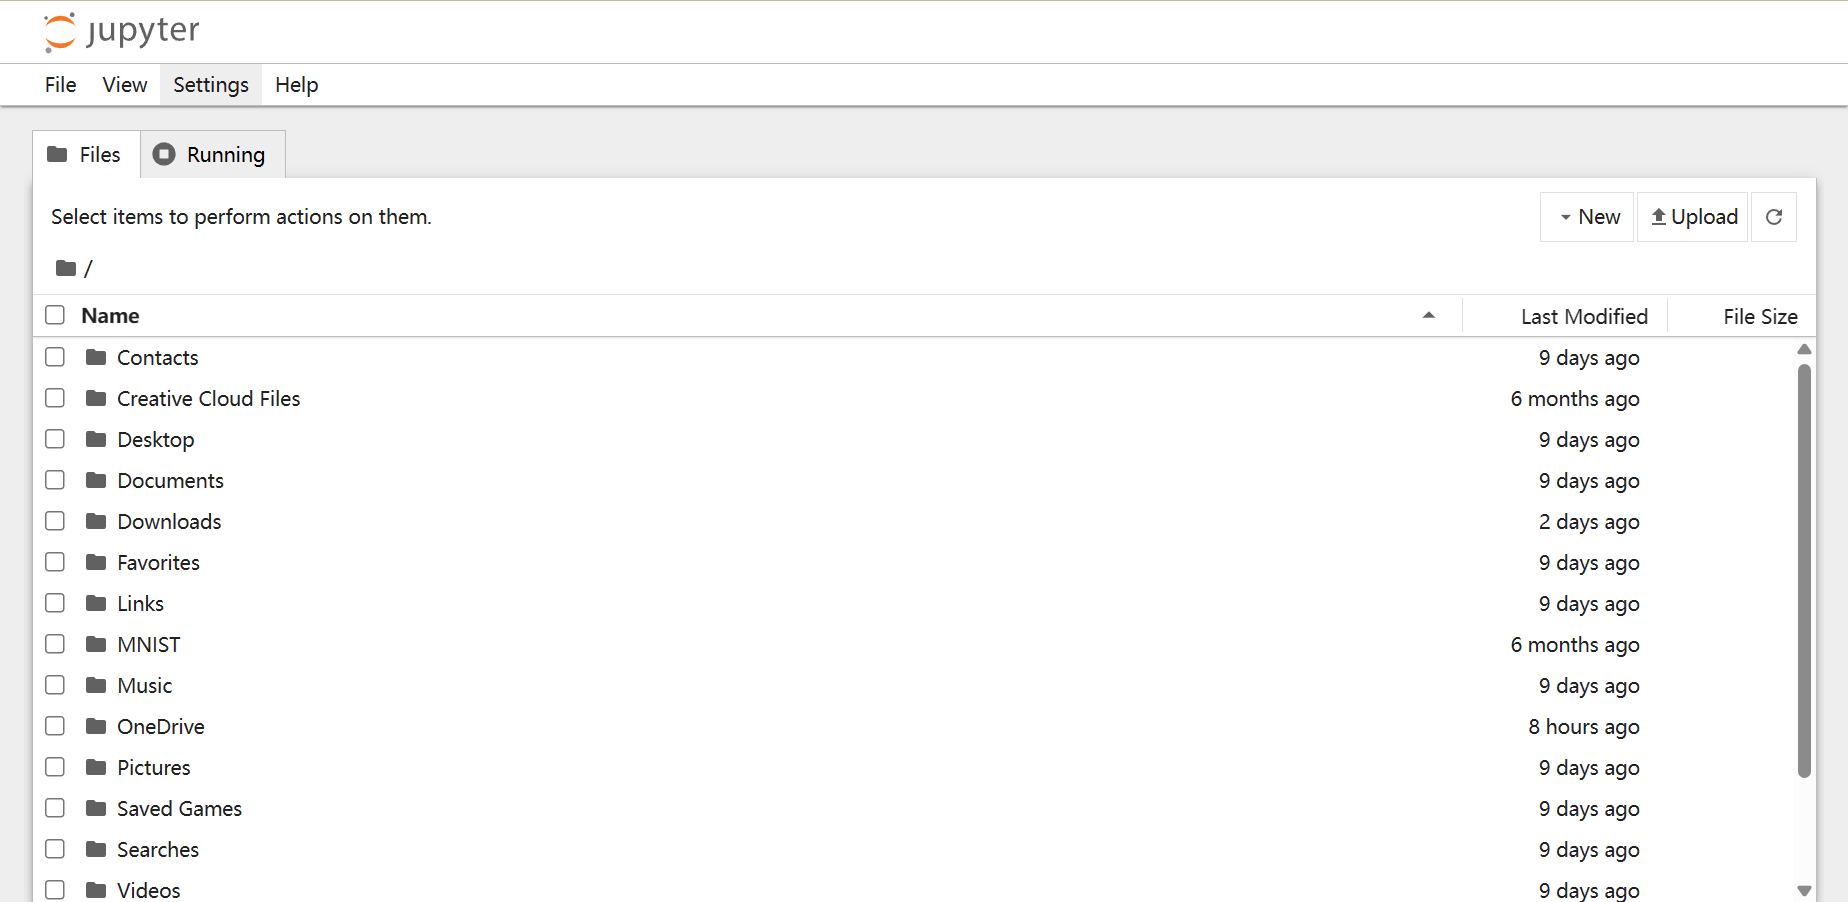
\includegraphics[width=\textwidth]{images/jupyter.png}
    \caption{Jupyter Notebook界面}
    \label{fig:jupyter}
\end{figure}

\subsection{高斯滤波器的生成}

如上文所述,高斯滤波器的卷积核可以通过多个一元高斯分布的乘积来生成。具体来说,可以通过以下代码来生成高斯滤波器的卷积核:

\begin{lstlisting}[style=Python]
def create_Gaussian_kernel(cutoff_frequency):
    # define 1d gaussion function
    def gaussion(x, mean, std):
        return 1 / (std * np.sqrt(2 * np.pi)) * np.exp(-0.5 * ((x - mean) / std) ** 2)

    def create_gaussian_naive(cutoff_frequency):
        """ Naive implementation of Gaussian kernel. """
        # define kernel size
        k = cutoff_frequency * 4 + 1
        kernel = np.zeros((k, k))

        # define mean and std
        mean = k // 2
        std = cutoff_frequency
        
        # calculate kernel for each pixel
        for i in range(k):
            for j in range(k):
                kernel[i, j] = gaussion(i, mean, std) * gaussion(j, mean, std)
        
        # normalize the kernel
        kernel /= np.sum(kernel)
        return kernel

    def create_gaussian_numpy(cutoff_frequency):
        """ Numpy implementation of Gaussian kernel. """
        ...
        # create 1d gaussion function
        x = np.arange(k)
        kernel_x = gaussion(x, mean, std)
        
        # create 2d gaussion function
        kernel = np.outer(kernel_x, kernel_x)
        ...
        return kernel

    # return create_gaussian_naive(cutoff_frequency)
    return create_gaussian_numpy(cutoff_frequency)
\end{lstlisting}

考虑到篇幅限制,部分重复代码被用省略号代替,完整代码可以在附录A中找到。上述代码中,首先定义了一维高斯函数\texttt{gaussion},然后提出了2种实现方式:

\begin{enumerate}
    \item \texttt{create\_gaussian\_naive}:通过循环来实现高斯滤波器的卷积核生成。具体来说,首先定义了卷积核的大小以及高斯分布的均值和标准差,然后遍历每个像素,通过2个不同维度的一元高斯分布的乘积得到结果,最后对卷积核进行归一化。
    \item \texttt{create\_gaussian\_numpy}:通过numpy来实现高斯滤波器的卷积核生成。具体来说,首先定义了卷积核的大小以及高斯分布的均值和标准差,然后通过numpy的\texttt{outer}函数来实现2个不同维度的一元高斯分布的乘积,最后对卷积核进行归一化。
\end{enumerate}

通过上述函数,在指定截止频率的情况下,可以生成高斯滤波器的卷积核。

\subsection{滤波操作的实现}

如上文所述,可以通过卷积操作来实现滤波操作。具体来说,可以通过以下代码来实现滤波操作:

\begin{lstlisting}[style=Python]
def my_imfilter(image, filter):
    # naive implementation
    def my_imfilter_naive(image, filter):
        """ Naive implementation of image filter, use for loop. """
        
        def apply_filter(patch, filter):
            pixel = 0
            # for each pixel
            for k in range(K):
                for j in range(J):
                    # multiply the pixel value with the filter value
                    pixel += patch[k, j] * filter[k, j]
            # the final pixel value is the sum of all the pixel value multiplied by the filter value
            return pixel
        
        M, N, C = image.shape
        K, J = filter.shape

        # padding image
        # (M, N, C) -> (M + 2 * P, N + 2 * P, C)
        pad_M, pad_N = K // 2, J // 2
        image_pad = np.zeros((M + 2 * pad_M, N + 2 * pad_N, C))
        image_pad[pad_M: M + pad_M, pad_N: N + pad_N, :] = image

        image_new = np.zeros((M, N, C))
        
        # for each pixel, ignore the boundary
        for m in range(M):
            for n in range(N):
                # for each channel
                for c in range(C):
                    # get image patch by using the current pixel (i, j) as the center
                    patch = image_pad[m: m + K, n: n + J, c]
                    image_new[m, n, c] = apply_filter(patch, filter)
        
        return image_new
    
    # ==================================================
    # numpy implementation, using matrix multiplication to accelerate the process
    def my_imfilter_numpy(image, filter):
        ...
        image_pad = np.pad(image, ((pad_M, pad_M), (pad_N, pad_N), (0, 0)), 'constant')

        # image to column
        # (M, N, C) -> (M * N * C, K * j)
        image_col = np.zeros((M * N * C, K * J))
        col_idx = 0
        for m in range(M):
            for n in range(N):
                for c in range(C):
                    patch = image_pad[m: m + K, n: n + J, c]
                    image_col[col_idx] = patch.flatten()
                    col_idx += 1
        
        # apply filter
        # (M * N * C, K * J) @ (K * J, 1) -> (M * N * C, 1)
        filter_col = filter.flatten()
        image_new_col = np.dot(image_col, filter_col)
        
        # reshape the image
        image_new = image_new_col.reshape((M, N, C))
        return image_new

    # ==================================================

    # numpy implementation, using stride trick to accelerate image to column
    def my_imfilter_numpy_stride_trick(image, filter):
        """ Numpy implementation of image filter, use matrix multiplication. """
        ...
        image_col = np.lib.stride_tricks.sliding_window_view(image_pad, (K, J, 1)).reshape((M * N * C, K * J))
        ...
        return image_new

    # ==================================================
    
    # fft implementation, faster but may have some error
    def my_imfilter_fft(image, filter):
        """ FFT implementation of image filter. """
        freq_filter = np.fft.fft2(filter, s=image.shape[:2])
        for c in range(image.shape[2]):
            freq_per_channel = np.fft.fft2(image[:, :, c])
            image[:, :, c] = np.fft.ifft2(freq_per_channel * freq_filter).real
        return image
    
    # return my_imfilter_naive(image, filter)
    # return my_imfilter_numpy(image, filter)
    return my_imfilter_numpy_stride_trick(image, filter)
    # return my_imfilter_fft(image, filter)
\end{lstlisting}

考虑到篇幅限制,部分重复代码被用省略号代替,完整代码可以在附录A中找到。上述代码中,提出了4种滤波操作的实现方式:

\begin{enumerate}
    \item \texttt{my\_imfilter\_naive}:通过循环来实现滤波操作。具体来说,首先对图像进行填充,然后遍历每个像素,通过应用卷积操作得到结果。卷积操作同样通过循环来实现,最后得到滤波后的图像。
    \item \texttt{my\_imfilter\_numpy}:通过numpy来实现滤波操作。具体来说,首先对图像进行填充,然后通过循环操作来实现图像到列的转换,最后通过numpy的矩阵乘法来实现卷积操作,最后还原原图像的尺寸。
    \item \texttt{my\_imfilter\_numpy\_stride\_trick}:通过numpy的\\ \texttt{sliding\_window\_view}函数来实现滤波操作。具体来说,首先对图像进行填充,然后通过numpy的\texttt{sliding\_window\_view}函数来实现卷积操作,最后得到滤波后的图像。
    \item \texttt{my\_imfilter\_fft}:通过FFT来实现滤波操作。具体来说,首先对滤波器进行傅里叶变换,然后对图像的每个通道进行傅里叶变换,最后通过频域的乘法来实现卷积操作,最后通过逆傅里叶变换得到滤波后的图像。
\end{enumerate}

通过上述函数,可以在指定图像和滤波器的情况下,实现滤波操作。

\subsection{混合图像的实现}

如上文所述,可以通过高通滤波器和低通滤波器的组合来实现混合图像的效果。具体来说,可以通过以下代码来实现混合图像的效果:

\begin{lstlisting}[style=Python]
def create_hybrid_image(image1, image2, filter):
    if image1.shape != image2.shape:
        # resize the larger image to the size of the smaller image using numpy
        image1_size = image1.shape[0] * image1.shape[1]
        image2_size = image2.shape[0] * image2.shape[1]
        if image1_size < image2_size:
            np.resize(image2, image1.shape)
        else:
            np.resize(image1, image2.shape)
    
    # get low pass by using the filter
    low_pass_image1 = my_imfilter(image1, filter)
    # get high pass by subtracting the low pass from the original image
    high_pass_image2 = image2 - my_imfilter(image2, filter)
    # hybrid image is the sum of low pass and high pass
    hybrid_image = low_pass_image1 + high_pass_image2
    
    # clip the pixel values
    hybrid_image = np.clip(hybrid_image, 0.0, 1.0)
    
    return low_pass_image1, high_pass_image2, hybrid_image
\end{lstlisting}

考虑到篇幅限制,部分重复代码被用省略号代替,完整代码可以在附录A中找到。函数\texttt{create\_hybrid\_image}接收两个图像和一个滤波器作为输入,然后通过低通滤波器提取第一个图像的低频信息,通过原图与低通滤波后的图像相减提取第二个图像的高频信息,最后将两者叠加在一起,即可得到混合图像。为了防止像素值超出范围,还需要对混合图像进行裁剪。通过上述函数,可以实现混合图像的效果。

\subsection{测试程序的运行}

在实现了上述函数后,可以在Jupyter Notebook中调用这些函数来测试程序的运行。如图\ref{fig:jupyter_run_all}所示,在Jupyter Notebook中打开\\\texttt{part1\_test\_filtering.ipynb}和\texttt{part1.ipynb}文件,然后点击"Restart the kernel and run all cells"按钮,即可运行测试程序。

\begin{figure}
    \centering
    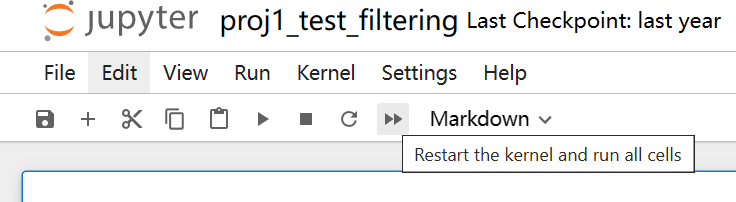
\includegraphics[width=\textwidth]{images/jupyter_run_all.png}
    \caption{Jupyter Notebook运行所有单元格}
    \label{fig:jupyter_run_all}
\end{figure}

运行成功后,可以看到测试程序的输出结果。

\section{实验结果与分析}

\subsection{图像滤波的结果}

图\ref{fig:jupyter_output}展示了\texttt{part1\_test\_filtering.ipynb}的运行结果,图中包含了原始图像、均值滤波器、Sobel滤波器、拉普拉斯滤波器处理后的图像,可以通过这些图像来观察滤波器作用于图像上的效果。具体来说:

\begin{figure}[htbp]
    \centering
    \subfloat[原始图像]{\includegraphics[width=0.3\textwidth]{images/data/1b_cat.bmp}}
    \subfloat[Identity滤波]{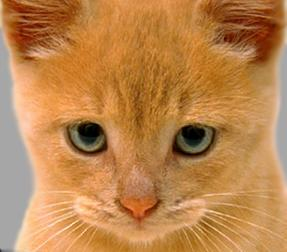
\includegraphics[width=0.3\textwidth]{images/part1/identity_image.jpg}}
    \subfloat[均值滤波]{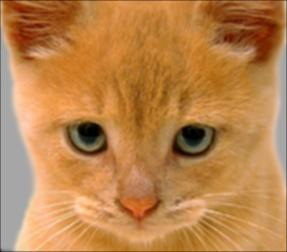
\includegraphics[width=0.3\textwidth]{images/part1/blur_image.jpg}}
    \\
    \subfloat[Sobel滤波]{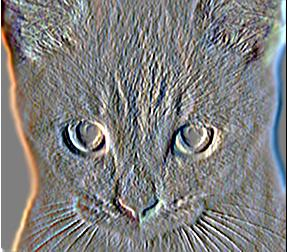
\includegraphics[width=0.3\textwidth]{images/part1/sobel_image.jpg}}
    \subfloat[拉普拉斯滤波]{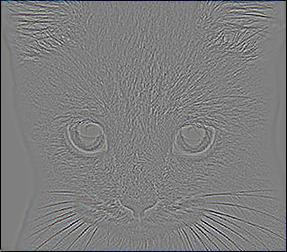
\includegraphics[width=0.3\textwidth]{images/part1/laplacian_image.jpg}}
    \subfloat[高通滤波]{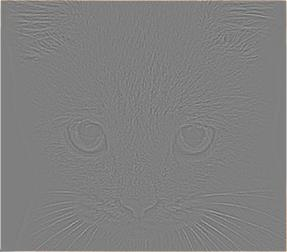
\includegraphics[width=0.3\textwidth]{images/part1/high_pass_image.jpg}}
    \caption{测试程序的输出结果}
    \label{fig:jupyter_output}
\end{figure}

\begin{enumerate}
    \item 子图(a)是原始图像。
    \item 子图(b)是Identity滤波器处理后的图像,由于滤波器被设置为中心为1,周围为0,因此图像不会发生变化。
    \item 子图(c)是均值滤波器处理后的图像,由于滤波器的每个元素被设置为和为1的均值,因此图像中每个像素会变成当前像素与周围像素的均值,即图像会变得模糊。
    \item 子图(d)是Sobel滤波器处理后的图像,由于滤波器左边的元素被设为负值,右边的元素被设为正值,因此图像中的每个像素会变成左边像素与右边像素的差值,突出垂直边缘信息。
    \item 子图(e)是拉普拉斯滤波器处理后的图像,由于滤波器中心为-4,周围为1,因此图像中的每个像素会变成当前像素与周围像素的差值,突出图像的边缘信息。
    \item 子图(f)是高通图像,是原始图像减去均值滤波器处理后的图像,由于均值滤波会模糊图像,因此原始图像与模糊图像的差值会突出图像中显著的细节信息。
\end{enumerate}

\subsection{图像混合的结果}

图\ref{fig:jupyter_output2}展示了\texttt{part1.ipynb}的运行结果,首先程序返回的验证结果均为True,证明程序编写无误。接下来,运行结果中包含了原始图像、高斯滤波器、滤波后的图像和混合图像,可以通过这些图像来观察滤波器作用于图像上的效果。具体来说:

\begin{figure}[htbp]
    \centering
    \subfloat[原始图像]{\includegraphics[width=0.2\textwidth]{images/data/1a_dog.bmp}}
    \subfloat[原始图像]{\includegraphics[width=0.2\textwidth]{images/data/1b_cat.bmp}}
    \subfloat[高斯滤波器]{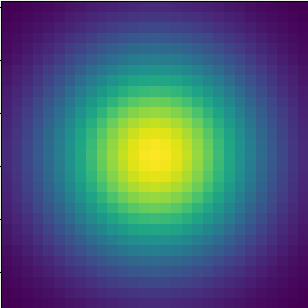
\includegraphics[width=0.2\textwidth]{images/gaussian.png}}
    \subfloat[低通图像]{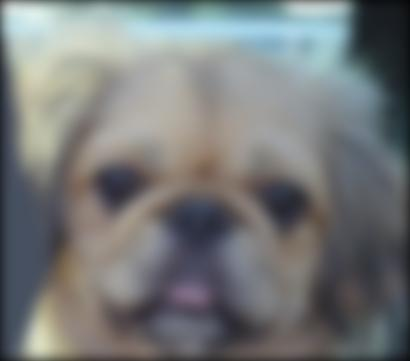
\includegraphics[width=0.2\textwidth]{images/part1/low_frequencies.jpg}}
    \subfloat[高通图像]{
\includegraphics[width=0.2\textwidth]{images/part1/high_frequencies.jpg}}
    \\
    \subfloat[混合图像]{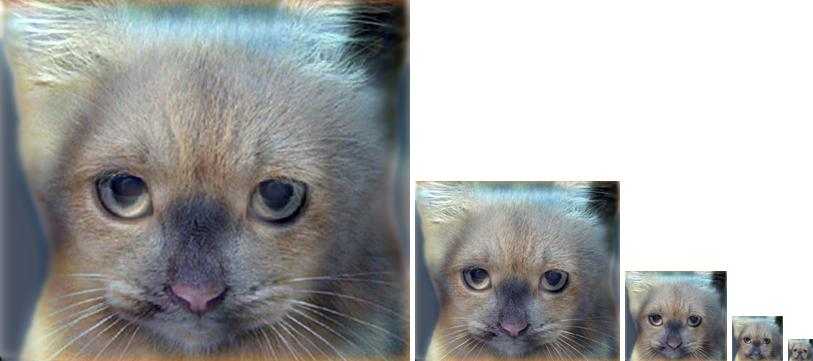
\includegraphics[width=\textwidth]{images/part1/hybrid_image_scales.jpg}}
    \caption{测试程序的输出结果}
    \label{fig:jupyter_output2}
\end{figure}

\begin{enumerate}
    \item 子图(a)、(b)是原始图像。
    \item 子图(c)是高斯滤波器,高斯滤波器被设置为中间大,周围小的二维高斯分布,因此可以起到平滑图像的作用。
    \item 子图(d)是低通图像,是原始图像与高斯滤波器处理后的图像的卷积结果,可以看到图像中的整体信息被保留。
    \item 子图(e)是高通图像,是原始图像减去低通图像,可以看到图像中的细节信息被突出。
    \item 子图(f)是混合图像,是低通图像和高通图像的相加,可以看到图像中的整体信息和细节信息被合并在一起。将图像按不同尺寸显示,可以看到图像越大,越容易看到高频信息(猫);图像越小,越容易看到低频信息(狗)。
\end{enumerate}

需要注意的是,基于FFT的卷积方式得到的结果与其他方法不同,并不能实现有效的图像混合。如图\ref{fig:fft}所示,通过FFT方式得到的混合图像与其他方式得到的混合图像有明显的差异,这是由于FFT是基于频域的角度来实现卷积,而空域到频域的转换会导致一些信息的丢失,如一些细节信息,因此在实际应用中需要根据具体情况选择合适的实现方式。基于FFT得到的完整结果可以在附录B中找到。

\begin{figure}[htbp]
    \centering
    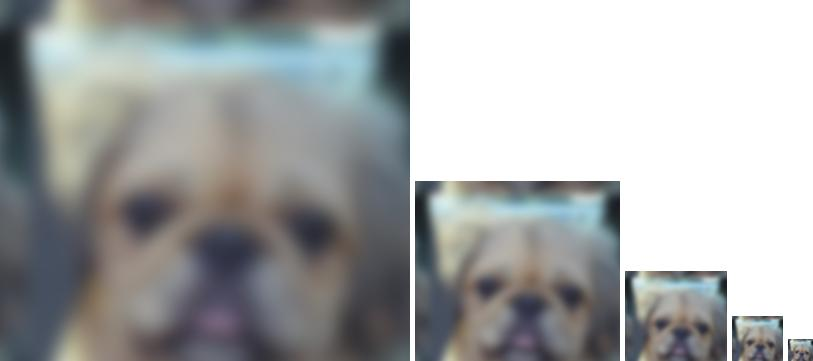
\includegraphics[width=\textwidth]{images/part1_fft/hybrid_image_scales.jpg}
    \caption{FFT得到的混合图像}
    \label{fig:fft}
\end{figure}

\subsection{运行效率的比较}

\texttt{part1.ipynb}中展示了混合操作的运行时间,以及与torch卷积操作的运行时间的比较。如表\ref{tab:time}所示,可以看出不同实现方式的运行时间有较大差异,其中Naive实现方式的运行时间最长,FFT实现方式的运行时间最短,但是结果存在误差。而Numpy和Numpy Kernel Trick的实现方式在运行时间和结果正确性上都有较好的表现,不过与Pytorch相比,仍然有一定的差距。

其中,高斯核生成操作的实现方式影响不大,而卷积操作的实现方式对运行时间有较大影响。这是因为卷积操作是整个混合图像生成过程中最耗时的操作,涉及5层循环:遍历图像的每个像素(行和列)、遍历图像的每个通道、遍历卷积核的每个像素(行和列)。因此,通过优化卷积操作的实现方式,可以显著提高运行效率。考虑到估计时间的误差,实际运行效率可能会有所不同,但是大致可以看出不同实现方式的运行效率的差异。

\begin{table}[htbp]
    \tabcolsep=8pt
    \centering
    \caption{运行时间的比较}
    \label{tab:time}
    \begin{tabular}{c|c|c|c}
        \hline
        高斯核生成操作 & 卷积操作 & 结果是否正确 & 耗时(秒) \\
        \hline
        \multirow{4}{*}{Naive} & Naive              & √ & 550.127 \\
                               & Numpy              & √ & 8.726 \\
                               & Numpy Kernel Trick & √ & 6.578 \\
                               & Numpy FFT          & × & 0.271 \\
        \hline
        \multirow{4}{*}{Numpy} & Naive              & √ & 549.535 \\
                               & Numpy              & √ & 7.483 \\
                               & Numpy Kernel Trick & √ & 5.109 \\
                               & Numpy FFT          & × & 0.277 \\
        \hline
        Pytorch                & Pytorch            & √ & 2.595 \\
        \hline
    \end{tabular}
\end{table}

\subsection{总结}

总的来说,本实验通过实现高斯滤波器的卷积核生成、滤波操作、混合图像等操作,验证了均值滤波、Sobel滤波、高通滤波等滤波器作用于图像上的效果,并通过高通滤波器和低通滤波器的组合来实现混合图像的效果。通过实验得出了如下结论:

\begin{enumerate}
    \item 滤波器是一种简单而有效的图像处理操作,通过简单定义不同的滤波器,就可以实现多样的图像处理效果,例如均值滤波器可以模糊图像,Sobel滤波器可以突出图像的边缘信息,拉普拉斯滤波器可以突出图像的边缘信息。
    \item 通过高通滤波器和低通滤波器的组合,可以实现混合图像的效果,即将图像的低频信息和高频信息分别提取出来,然后叠加在一起。混合图像可以实现有趣的视觉效果,例如随着观察距离的变化,图像的低频和高频信息会以不同的形式呈现。图像越近,越容易看到高频信息;图像越远,越容易看到低频信息。
    \item 卷积的实现方式有多种,包括循环、矩阵相乘、利用numpy内置函数、傅立叶快速卷积等方式。不同的实现方式有不同的运行效率。其中循环的运行效率非常低下,傅立叶快速卷积虽然运行效率较高,但可能会有一些误差,因此在实际应用中需要根据具体情况选择合适的实现方式。
\end{enumerate}

\section{实验结论}

本实验讲述了滤波器和卷积操作的原理,以不同方式实现了滤波器生成、卷积、混合图像等操作,验证了均值滤波、Sobel滤波、高通滤波等滤波器作用于图像上的效果,并通过高通图像和低通图像的组合来实现混合图像的效果,还对不同实现方式的运行效率进行比较。通过本次实验,我对图像滤波的原理和实现方法有了更深入的了解,掌握了图像滤波的基本操作。

对于本实验,我认为还有以下几点可以改进的地方:

\begin{enumerate}
    \item 在实现滤波器生成时,可以尝试更多的滤波器的生成方式,例如通过方差不相等的高斯分布函数的乘积来生成高斯滤波器的卷积核,或者协方差不为0的高斯分布函数的乘积来生成多维高斯滤波器的卷积核,并观察不同滤波器对图像的影响。
    \item 在实现混合图像时,可以尝试更多的滤波器组合,例如通过不同的高通滤波器和低通滤波器的组合,来实现更多样的混合图像效果。
\end{enumerate}

\appendix

\section{完整代码}

\label{appendix:code}

\begin{lstlisting}[style=Python]
import numpy as np


def compute_feature_distances(features1, features2):
    """
    This function computes a list of distances from every feature in one array
    to every feature in another.
    Args:
    - features1: A numpy array of shape (n,feat_dim) representing one set of
      features, where feat_dim denotes the feature dimensionality
    - features2: A numpy array of shape (m,feat_dim) representing a second set
      features (m not necessarily equal to n)

    Returns:
    - dists: A numpy array of shape (n,m) which holds the distances from each
      feature in features1 to each feature in features2
    """
    mode = 'euclidean'

    # Euclidean distance
    # D = \sqrt{\sum_{i=1}^{D} (x_i - y_i)^2}
    # (N, 1, D) - (1, M, D) -> (N, M, D) -> (N, M)
    if mode == 'euclidean':
        return np.sqrt(np.sum((features1[:, None] - features2) ** 2, axis=2))

    # Manhattan distance
    # D = \sum_{i=1}^{D} |x_i - y_i|
    if mode == 'manhattan':
        return np.sum(np.abs(features1[:, None] - features2), axis=2)

    # Chebyshev distance
    # D = \max_{i=1}^{D} |x_i - y_i|
    if mode == 'chebyshev':
        return np.max(np.abs(features1[:, None] - features2), axis=2)
    
    # Minowski distance
    # D = \left( \sum_{i=1}^{D} |x_i - y_i|^p \right)^{1/p}
    if mode == 'minowski':
        p = 3
        return np.sum(np.abs(features1[:, None] - features2) ** p, axis=2) ** (1 / p)


def match_features(features1, features2, x1, y1, x2, y2):
    """
    This function does not need to be symmetric (e.g. it can produce
    different numbers of matches depending on the order of the arguments).

    To start with, simply implement the "ratio test", equation 4.18 in
    section 4.1.3 of Szeliski. There are a lot of repetitive features in
    these images, and all of their descriptors will look similar. The
    ratio test helps us resolve this issue (also see Figure 11 of David
    Lowe's IJCV paper).

    You should call `compute_feature_distances()` in this function, and then
    process the output.

    Args:
    - features1: A numpy array of shape (n,feat_dim) representing one set of
      features, where feat_dim denotes the feature dimensionality
    - features2: A numpy array of shape (m,feat_dim) representing a second
      set of features (m not necessarily equal to n)
    - x1: A numpy array of shape (n,) containing the x-locations of features1
    - y1: A numpy array of shape (n,) containing the y-locations of features1
    - x2: A numpy array of shape (m,) containing the x-locations of features2
    - y2: A numpy array of shape (m,) containing the y-locations of features2

    Returns:
    - matches: A numpy array of shape (k,2), where k is the number of matches.
      The first column is an index in features1, and the second column is an
      index in features2
    - confidences: A numpy array of shape (k,) with the real valued confidence
      for every match

    'matches' and 'confidences' can be empty e.g. (0x2) and (0x1)
    """
    
    def mean_distance_filter(dists, alpha):
        """
        Generate mask for matching features based on mean distance.
        Params:
        - dists (M,)
        Return:
        - mask (M,)
        """
        mean_dist = np.mean(dists)
        std_dist = np.std(dists)
        return dists < mean_dist - alpha * std_dist
    
    
    def mean_cosine_filter(cosines, alpha):
        """
        Generate mask for matching features based on mean cosine similarity.
        Params:
        - cosines (M,)
        Return:
        - mask (M,)
        """
        mean_cosine = np.mean(cosines)
        std_cosine = np.std(cosines)
        return cosines > mean_cosine + alpha * std_cosine
    
    
    def dist_ratio_filter(best_match_dists, second_match_dists, thresh):
        """
        Generate mask for matching features based on distance ratio.
        Params:
        - best_match_dists (M,)
        - second_match_dists (M,)
        Return:
        - mask (M,)
        """
        return (best_match_dists / second_match_dists) < thresh
    
    
    def cross_validation_filter(best_matches, inv_best_matches):
        """
        Generate mask for matching features based on cross validation.
        Params:
        - best_matches (M,): best matches for features1, elements are indices of features2
        - inv_best_matches (N,): best matches for features2, elements are indices of features1
        Return:
        - mask (M,)
        """
        return inv_best_matches[best_matches] == np.arange(best_matches.shape[0])
    
    
    def spatial_filter(shifts, cosine_thresh, dist_thresh):
        """
        Generate mask for matching features based on shifts.
        Params:
        - shifts (M, 2): shifts of features1 to features2
        Return:
        - mask (M,)
        """
        # cosine mask
        # (1, 2)
        mean_direction = np.mean(shifts, axis=0, keepdims=True)
        # (M, 2), (1, 2) -> (M, 2)
        cosine = np.sum(shifts * mean_direction, axis=1) / (np.linalg.norm(shifts, axis=1) * np.linalg.norm(mean_direction, axis=1))
        cosine_mask = cosine > cosine_thresh

        # distance mask
        # (M,)
        dists = np.linalg.norm(shifts, axis=1)
        mean_dist = np.mean(dists)
        std_dist = np.std(dists)
        # between mean - std and mean + std
        dist_mask = (dists > mean_dist - dist_thresh * std_dist) & (dists < mean_dist + dist_thresh * std_dist)

        # return cosine_mask
        return cosine_mask & dist_mask
    
    
    def ranasc_filter():
        """
        Generate mask for matching features based on RANSAC.
        """
        pass

    mode = 'euclidean'
    dist_alpha = 0.1
    cosine_alpha = 0.7
    ratio_thresh = 0.8
    spatial_cosine_thresh = 0.6
    spatial_dist_thresh = 1.0
    
    print('Computing distances...')
    # (M, N)
    dists = compute_feature_distances(features1, features2)

    cosines = np.dot(features1, features2.T) / (np.linalg.norm(features1) * np.linalg.norm(features2))
    
    best_matches = np.argmin(dists, axis=1)
    inv_best_matches = np.argmin(dists, axis=0)

    best_match_dists = dists[np.arange(dists.shape[0]), best_matches]
    second_match_dists = dists[np.arange(dists.shape[0]), np.argsort(dists, axis=1)[:, 1]]
    best_match_cosines = cosines[np.arange(cosines.shape[0]), best_matches]

    if best_match_dists.shape[0] < 100:
        inds1, inds2 = np.arange(features1.shape[0]), best_matches
        matches = np.stack([inds1, inds2], axis=1)
        confidences = 1 / best_match_dists
        return matches, confidences
    
    dist_mask = mean_distance_filter(best_match_dists, dist_alpha)
    print('Distance filter dropped:', np.sum(~dist_mask))

    cosine_mask = mean_cosine_filter(best_match_cosines, cosine_alpha)
    print('Cosine filter dropped:', np.sum(~cosine_mask))

    ratio_mask = dist_ratio_filter(best_match_dists, second_match_dists, ratio_thresh)
    print('Ratio filter dropped:', np.sum(~ratio_mask))

    cross_val_mask = cross_validation_filter(best_matches, inv_best_matches)
    print('Cross validation filter dropped:', np.sum(~cross_val_mask))

    mask = dist_mask & cosine_mask & ratio_mask & cross_val_mask
    inds1, inds2 = np.arange(features1.shape[0]), best_matches
    matches = np.stack([inds1[mask], inds2[mask]], axis=1)
    confidences = 1 / best_match_dists[mask]

    # (M,) -> (M',) 
    x1, y1 = x1[matches[:, 0]], y1[matches[:, 0]]
    x2, y2 = x2[matches[:, 1]], y2[matches[:, 1]]
    shifts_x = x1 - x2
    shifts_y = y1 - y2
    shifts = np.stack([shifts_x, shifts_y], axis=1)

    spatial_mask = spatial_filter(shifts, spatial_cosine_thresh, spatial_dist_thresh)
    print('Spatial filter dropped:', np.sum(~spatial_mask))

    matches = matches[spatial_mask]
    confidences = confidences[spatial_mask]
    
    return matches, confidences
\end{lstlisting}

\end{document}
